\documentclass[draftclsnofoot,onecolumn,letterpaper,10pt]{IEEEtran}

\usepackage{geometry}
\geometry{textheight=9.5in, textwidth=7in}

\usepackage{float}
\usepackage{algorithm2e}
\usepackage{pgfgantt}
\usepackage{booktabs}
\usepackage{graphicx}
\graphicspath{{images/}}

\usepackage{listings}
% Default fixed font does not support bold face
\DeclareFixedFont{\ttb}{T1}{txtt}{bx}{n}{10} % for bold
\DeclareFixedFont{\ttm}{T1}{txtt}{m}{n}{10}  % for normal

% Custom colors
\usepackage{color}
\definecolor{mygreen}{rgb}{0,0.6,0}
\definecolor{mygray}{rgb}{0.5,0.5,0.5}
\definecolor{mymauve}{rgb}{0.58,0,0.82}

\lstset{%
  backgroundcolor=\color{white},   % choose the background color; you must add \usepackage{color} or \usepackage{xcolor}; should come as last argument
  basicstyle=\footnotesize,        % the size of the fonts that are used for the code
  breakatwhitespace=false,         % sets if automatic breaks should only happen at whitespace
  breaklines=true,                 % sets automatic line breaking
  captionpos=b,                    % sets the caption-position to bottom
  commentstyle=\color{mygreen},    % comment style
  extendedchars=true,              % lets you use non-ASCII characters; for 8-bits encodings only, does not work with UTF-8
  frame=R,	                   % adds a frame around the code
  keepspaces=true,                 % keeps spaces in text, useful for keeping indentation of code (possibly needs columns=flexible)
  keywordstyle=\color{blue},       % keyword style
%  language=Python,                 % the language of the code
  morekeywords={self},           % if you want to add more keywords to the set
  numbers=left,                    % where to put the line-numbers; possible values are (none, left, right)
  numbersep=0em,                   % how far the line-numbers are from the code
  numberstyle=\tiny\color{mygray}, % the style that is used for the line-numbers
  rulecolor=\color{black},         % if not set, the frame-color may be changed on line-breaks within not-black text (e.g. comments (green here))
  showspaces=false,                % show spaces everywhere adding particular underscores; it overrides 'showstringspaces'
  showstringspaces=false,          % underline spaces within strings only
  showtabs=false,                  % show tabs within strings adding particular underscores
  stepnumber=1,                    % the step between two line-numbers. If it's 1, each line will be numbered
  stringstyle=\color{mymauve}     % string literal style
}
\newcommand{\subparagraph}{}
\usepackage{titlesec}

\begin{document}
\begin{center}
	{\huge\textbf{Senior Software Engineering Design Group 7}}
	\vspace{1cm}

	{\Huge\textbf{brew.ai Progress Report -- Spring Term}}

	\vspace{2cm}
	\textbf{Connor Yates}\\yatesco@oregonstate.edu

	\textbf{Aravind Parasurama}\\parasura@oregonstate.edu

	\textbf{Cody Holliday}\\hollidac@oregonstate.edu

	\vspace{2cm}
	{\Large CS 463, Spring 2017}
	\vspace{1cm}
\end{center}

\newpage
\tableofcontents
\newpage

\section{Purposes and Goals}
\subsection{Project Purpose}
Brew.ai is a hardware and software solution for automated brewing of mead or beer.
Currently, home brewing requires a lot of time, knowledge, and patience.
As such, it is not accessible to amateurs, and brew.ai seeks to solve this problem.
From amateurs to professional brewers, we want brew.ai to be useful by automating the brewing process and helping brewers make better tasting products.

\subsection{Project Goals}
At the end of the project, we look to produce a physical device that contains the necessary electronics and software to control the brewing process.
The brew.ai device itself is a skeleton that will fit over a brewing container and will have various modules incorporated in it.
The device will monitor and control temperature, send and receive commands/data to and from the Android application, and monitor fermentation status.
From the perspective of a user, setup will be essentially plug-and-play.
No technical knowledge is needed beyond knowing how to pair a Bluetooth device an Android device, open an app, and put ingredients into a bucket.
brew.ai also will improve on its recipe over time by leveraging the power of reinforcement learning and the users own feedback on the product it creates.
A main goal of this project is creating a product with the ability to learn from each batch, and improve its performance.

\section{Current Project Status}

\subsection{Hardware\\{\em\textbf{Aravind Parasurama}}}
\subsubsection{Overview}
brew.ai hardware is modular, flexible, and scalable.
The current testing hardware is a generic large mason jar with a tight-sealing
electronic case, however the brew.ai platform can easily work with setups ranging
from what is used for testing to a professional brewing operation with multiple
brews being automated.
Currently, another prototype is being built that utilizes a glass carboy form factor,
proving the versatility of the brew.ai platform.
The hardware components can be categorized as the main controller element, and
everything else.
For this demo, the microcontroller of choice was originally the AVR ATmega32u4, which provides
us with a nice range of GPIO, PWM and ADC pins to work with when broken out.
Now, the system has been simplified to utilize the Raspberry Pi that hosts the AI for module
control and reading.
The Raspberry Pi will execute commands received from the AI, and send
sensor data to the AI.
Sensors are plug-and-play as per the user's discretion, however the crucial elements
for operation are the heating and cooling element, the water table sensor, and
the thermometer.
As the heating element requires a lot of power for continous operation, the brew.ai
hardware will require a consistent power source.

\subsubsection{Current Status}
The first hardware prototype is completed.
It is powered by a Raspberry Pi, and has various sensors plugged into it, and a heating and
stirring module set up as well.
Android software linkage is complete, and data readouts display on Androidl
Currently, brew testing is taking place  with the first hardware prototype.
A second hardware prototype based on a glass carboy brewing setup is currently 
being built, and will be ready for expo.

\begin{figure}
\label{fig:hw1}
\caption{The first device protoype brewing some mead}
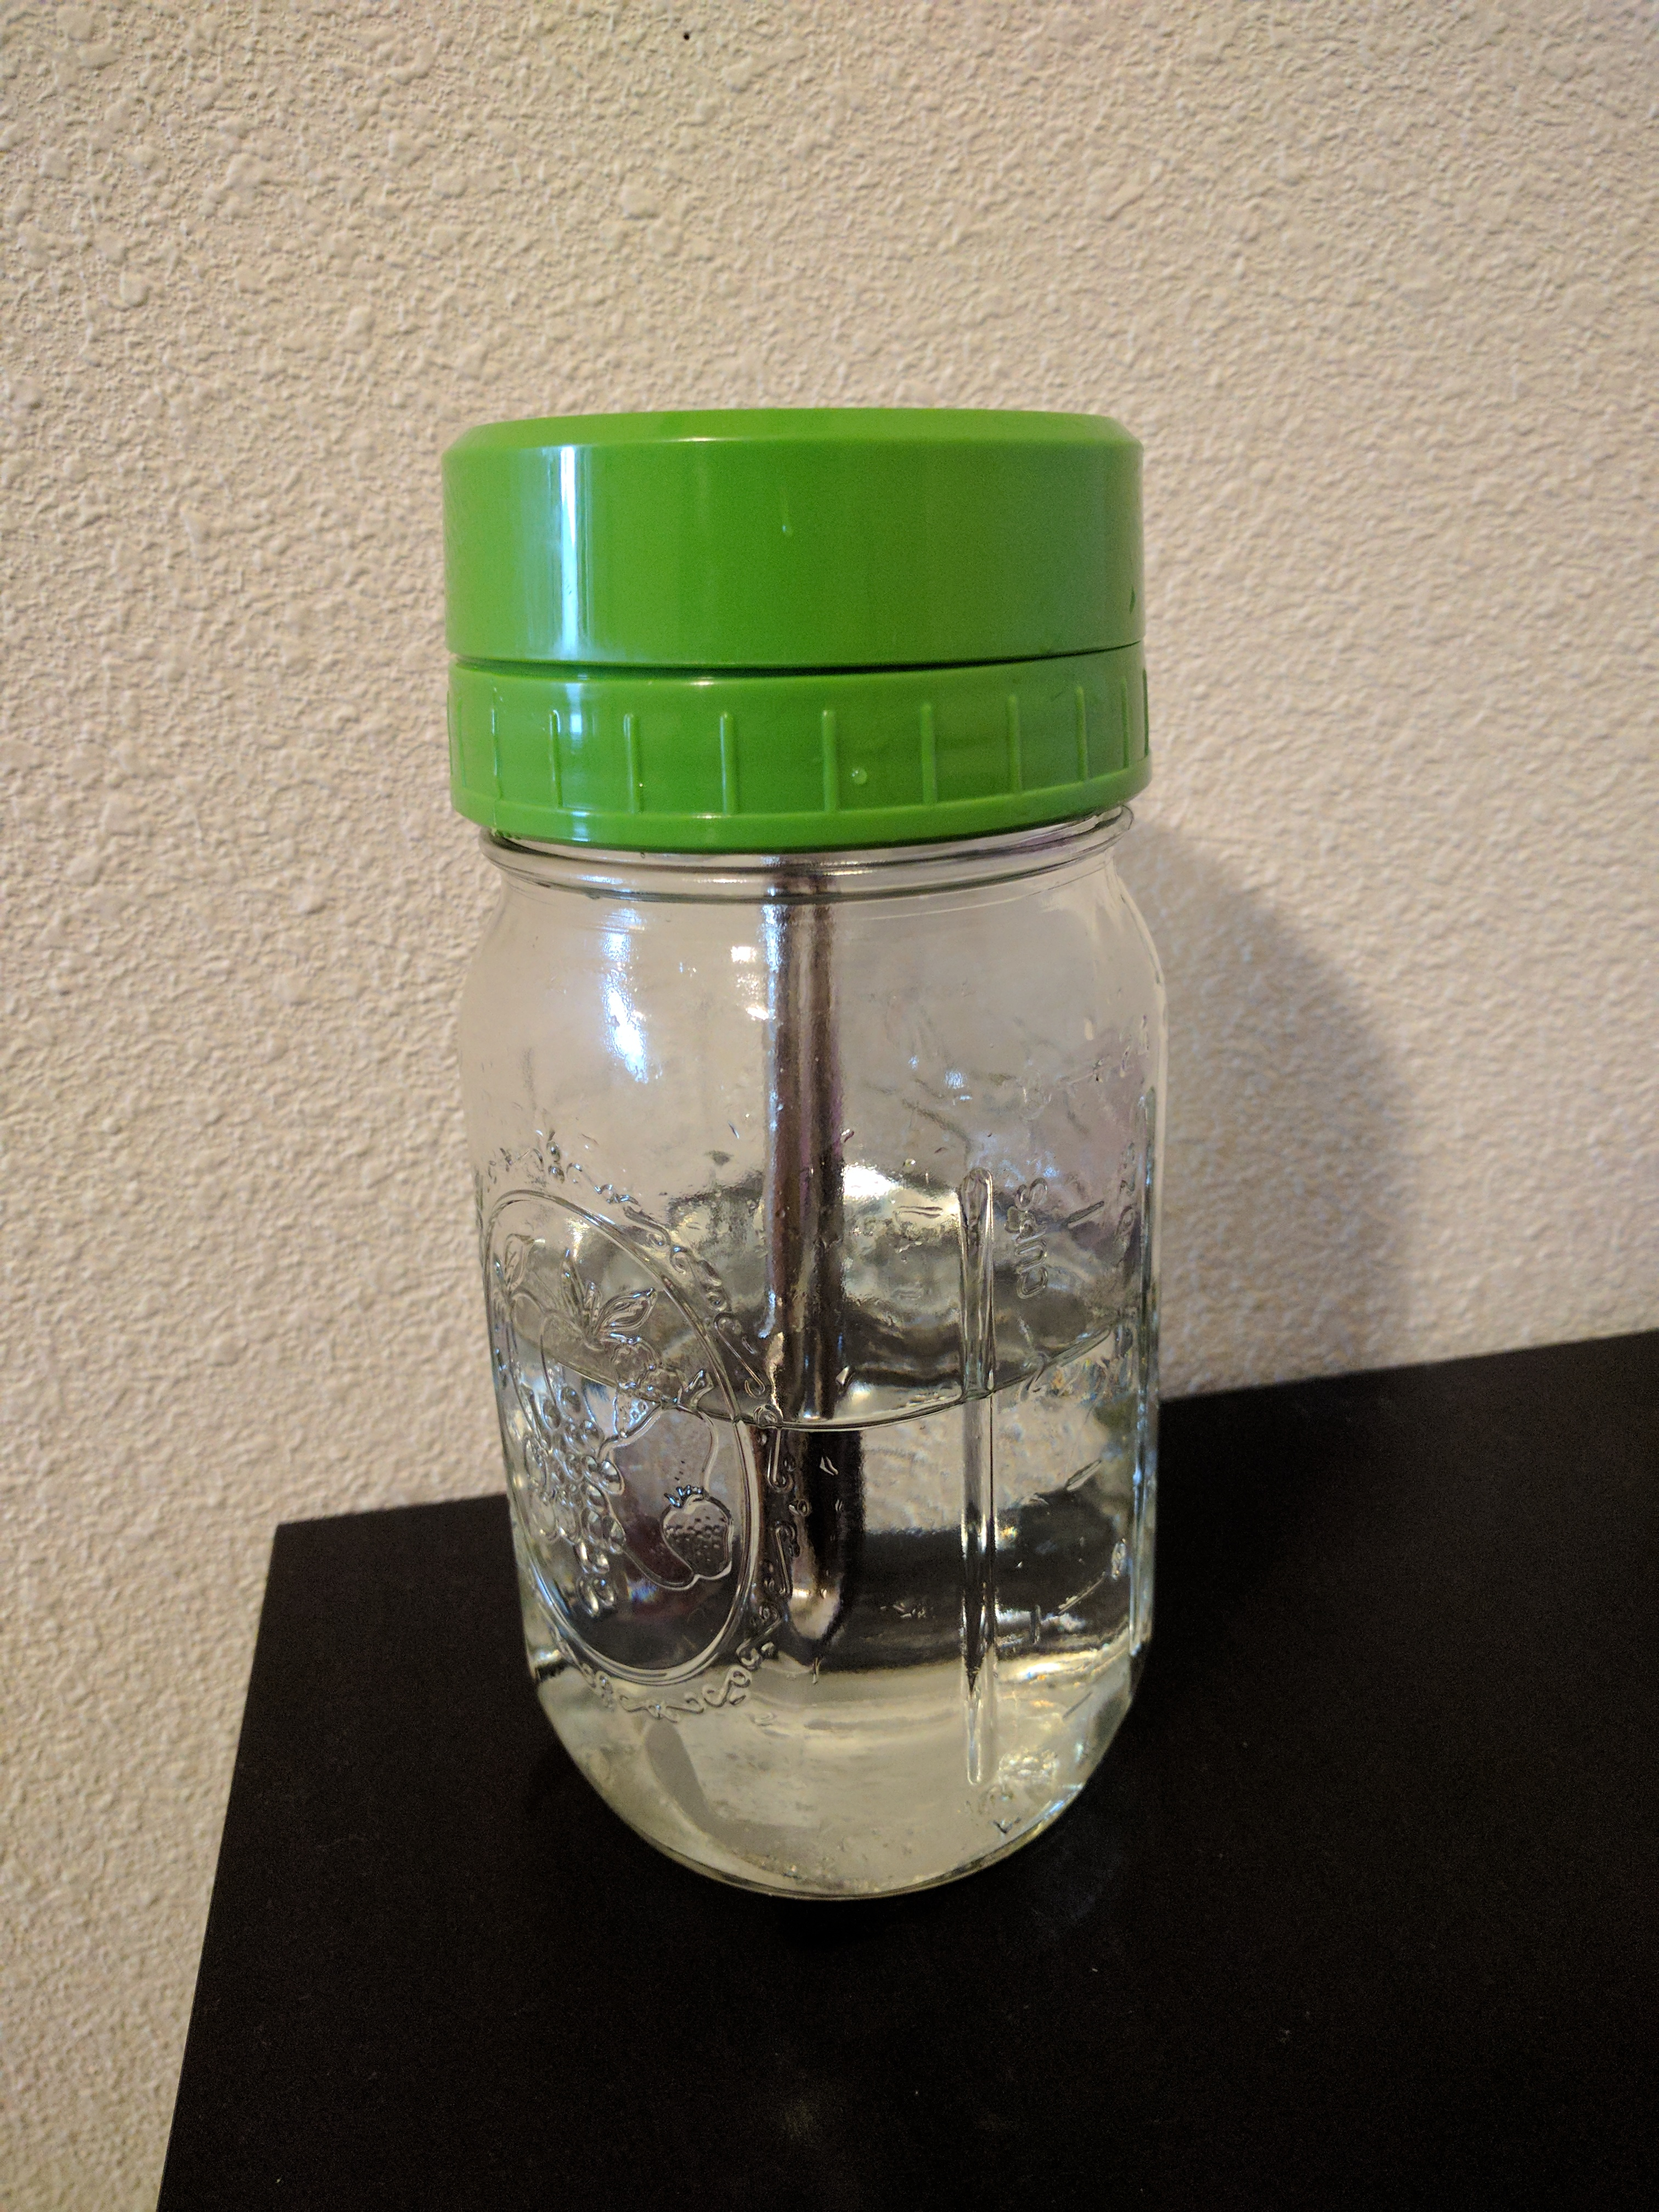
\includegraphics[width=\linewidth]{hw1.eps}
\end{figure}

\subsubsection{Tasks Left}
Construction of the second hardware prototype before expo is the biggest priority, along
with building a nice looking case for the first hardware prototype.
Otherwise, the only task is to continue brew testing.

\subsubsection{Roadblocks}
Finding a heating/stirring device to power the second hardware prototype was difficult, considering
the cost of one of those devices.
Otherwise, roadblocks have been minor, and limited to small hardware fixes to issues exposed during
brew testing.

\subsection{Android Interface\\{\em\textbf{Cody Holliday}}}
The Android app is almost feature complete. Significant progress was made during this term, but there was not enough time to complete it.


\subsubsection{Work Done and Roadblocks}
The work done this term included implementation of the survey after the brewing session, a pre-brewing activity, and a visual redesign of the app.
The pre-brewing activity collects information from the user about the ingredients as well as how the hardware should act.
This data is sent to the Raspberry Pi. After that the app continues in normal brewing mode.
I reworked the design for the main brewing activity to allow the users to see the sensor data separated by type.
In addition, the user can scroll through the graphs while still having the main buttons locked to the top.
After the brewing is completed, the user survey opens. 
Designing this activity was a painstaking process as this was the first redesign I did. I learned the best practice for design through trial and error.
The survey asks the user to describe the brew and whether or not they liked it.

The main roadblock for this entire process was design.
I went through a couple designs before I understood how to use the different containers and layouts available in the Android XML.



\subsubsection{Work Left Undone}
According to the client requirements there is only one thing left undone.
The pre-brewing section does send the data to the main brewing activity to be processed, but it never actually uses it.
It only uses it as a condition to begin the main brewing loop.

According to a previous app design, there is a lot not finished.
The user cannot recall the data from previous batches. There is no settings button for the user to use.
All the little intermediate screens for brewing are not implemented, and the brewing activity is the same as the main activity.
However, these are not in the client requirements. They were only in the progress report from winter term.

\subsubsection{Interesting Code}
I think the most clever code I wrote on this project had to do with the satisfaction buttons for each section on the user survey.
The buttons are actually radio buttons with their dots hidden.
\lstinputlisting[language=XML,firstline=333,lastline=342,caption={The emoji radio button in XML.}]{code/content_survey.xml}
Then I set the text of the radio buttons to the unicode values of three emojiis: happy, neutral, and sad.
\lstinputlisting[language=XML,firstline=16,lastline=18,caption={The unicode values for the emojiis.}]{code/strings.xml}
After that I created a color theme to change the alpha levels of the emojiis so that faces that weren't selected showed up gray.
\lstinputlisting[language=XML,firstline=1,lastline=6,caption={The color theme used for the emojiis.}]{code/radioselector.xml}
Basically it is a normal radio button group, but it looks completely different.
\newpage
\vfill
\subsubsection{App Design}
The app has three activities: main (Middle), pre-brew (Left), and the survey (Right).
The main activity is both the main activity as well as the brewing activity.
After the user connects using the connect button in the top right of the main activity, they press start which will take them to the pre-brewing activity(Left).
The user enters their ingredient amounts, then presses submit. After that the app goes back to the main activity and shows data streaming from the Pi.
After the brew ends, the user is taken to the survey activity where they enter information about the batch.
\begin{figure}
\label{fig:code}
\caption{These are the activities in the app.}
\includegraphics[scale=0.15]{brewing.eps}
\end{figure}

\vfill
\clearpage


\subsection{Artificial Intelligence\\{\em\textbf{Connor Yates}}}
\subsubsection{AI Review and Purpose}
The artificial intelligence aspect of this project is to create an autonomous agent which watches over the brewing process.
The agent will have the ability to read data from sensors immersed in the brew, and act upon its decisions.
Available actions are a stirring element, a heating element, and a trigger to stop the brewing process.

Instead of hand-coding a specific policy based on historical data, we elected to use reinforcement learning.
Specifically, we will use Q-learning with experience replay to train a neural network to gauge what actions should be taken when presented with a representation of the world.
Q-learning traditionally uses a table to store Q-values for a finite set of state-actions pairs.
We will represent our brewing process as a 4-dimensional state storing the current temperature, specific gravity, $CO_2$ level, and time.
These variables are continuous, and have a potentially infinite range.
Instead of attempting to manually bin their continuous domain into a discreet one, we will use a neural network to stand in place of the Q-table.
Neural networks are general function approximators, and have been shown to be able to approximate the function encoded by the Q-table.
This method will provide the structure for an intelligent, autonomous agent which learns from its environment.

In order to test the performance and robustness of the AI, we are considering creating a simple simulator of a brewing system, based on simple physics principles.
This system will allow us to create basic, but meaningful test data with which to train the AI on.
The need for this secondary system is not yet cemented, but I will be proceeding as if it is needed.

\subsubsection{AI Progress}
In the winter progress report, the main hurdle left was data collection and training. This is currently an ongoing process, as brewing is a time-intensive process. However, the AI section has been finished for some time, and subsequently no development has been needed in this section. The following sections detail the state of AI section of the project.

\subsubsection{Learning Agent}
The first two items were completed handily, and the third is currently underway. The next two sections are examinations of interesting code sections, to explain the solution to the first two problems.
The learning agent was quickly completed one weekend after the winter progress report. The most difficult function to write was the q-update function, where the learning occurs. This function is provided in Listing~\ref{lst:q-update}.
\lstinputlisting[language=Python,firstline=41,lastline=86,caption={Q-Update function to learn from the current reward and history of actions}]{code/qlearning.py}\label{lst:q-update}
The method works by assembling the experience-replay memory, a list of state-action-state transitions from the current brewing run. It pairs this with the reward from the user, and uses the Bellman update function (line 21) to calculate the new best-action that the agent should take when it finds itself in a given state. With the action the current network provides and the new action it should take, we can perform standard backpropogation to train the network to output the new value (lines 41-45). By doing this repeatedly, the neural network learns an optimal action-selection policy. An analysis of the learning for the simple simulator will be given in Section~\ref{sec:AI-Results}.

After this code was finished, the necessary dependencies were compiled onto the Raspberry Pi, and the learning agent was tested for basic functionality and the ability to run on the Raspberry Pi. The agent can make a single decision every few minutes, since it has a relatively slow processor and no GPU to speed up the neural network math. However, unlike many applications of machine learning this slow response time is not an issue for this project, as brewing is a slow, steady process that can take weeks.

\subsubsection{Simple Simulator}
This simulator was a very simple tested for ensuring the artificial intelligence was functioning correctly. It is comprised of a Python class object, which internally holds four variables: time, temperature, $CO_2$ levels, and specific gravity. Together, these variables represent the state of the brewing system. The simulator also keeps track of the reward, which is a measure of how successful and tasty the final product would be. This is determined by short functions which provide optimal bounds for values of the state variables. For example, if the temperature becomes too high or too low, the fermentation process would end prematurely. The code in Listing~\ref{lst:temp_reward} decrements the reward if it strays from these bounds. It also provides positive rewards for being inside the ``optimal'' bounds.
\lstinputlisting[language=Python,firstline=17, lastline=27,caption={Reward changes for the temperature variable}]{code/simulator.py}\label{lst:temp_reward}

\subsubsection{Results}\label{sec:AI-Results}
The agent was trained to provide actions to the simulator, which would provide the next state to the agent. It would provide the reward at the end of a trial brewing, from which the agent would perform a learning update. After learning from the trial, the agent would run another trial. The agent is able to learn a successful policy over the course of 5000 trials. This is shown by the reward, a measure of performance, at each trial in Figure~\ref{fig:trial_graph}. 
\begin{figure}[h]
\label{fig:trial_graph}
\caption{Learning is shown by the reduction of sub-par rewards over the course of the 5000 trials. Note that the simulator has discreet reward increments, resulting in the stratified nature of the graph. Additionally, each trial has random exploration movements at the beginning preventing a single coalesced result toward the end of the trials.}
\includegraphics[width=\linewidth]{trial_reward.eps}
\end{figure}

\end{document}
